

\textbf{I}. Найдём уровни энергии и волновые функции связанных состояний ($E<0$) частицы в поле
\begin{equation*}
    U(x) = - \frac{\hbar^2 \kappa_0}{m} \left( \bp
        \delta(x+a)+\delta(x-a)
    \right).
\end{equation*}
Гамильтониан системы и стационарное уравнение Шрёдингера:
\begin{equation*}
    H = - \frac{\hbar^2 \partial_x^2}{2m} + U(x),
    \hspace{5 mm}
    - \frac{\hbar^2 \partial_x^2}{2m} \psi(x) + U(x) \psi(x) = - |E| \psi(x),
\end{equation*}
далее считая $E = - E$, будем решать уравнение
\begin{equation*}
    \psi''(x) - \frac{2m}{\hbar^2} (U(x) + E) \psi(x) = 0.
\end{equation*}
В местах, где не происходит скачков производной подходит в качестве решения экспонента, так что будем искать решение в виде
\begin{equation*}
    \psi(x) = \left\{\begin{aligned}
        &A e^{\kappa (x+a)}, &x<-a \\
        &B e^{-\kappa(x+a)} + C e^{\kappa(x-a)}, &|x| < a \\
        &D e^{-\kappa (x-a)}, &x > a.
    \end{aligned}\right.
\end{equation*}
где введено $\kappa^2 = {2 m E}/{\hbar^2}$. 

Можно было бы заметить, что потенциал симметричен, а значит можно искать решение уравнения Шредингера, как собственные функции оператора инверсии: четные и нечетные решения ($A=D,\, B=C$ и $A=-D,\, B=-C$), но мы пойдём другим путём, чтобы посмотреть, как из уравнений вылезет симметрия задачи.


Чтобы найти $\psi(x)$ запишем условия непрерывности и, интегрируя стационарное уравнение Шредингера, уравнение на скачок производной:
\begin{equation*}
    \left.\begin{aligned}
        \psi(-a+\varepsilon) &= \psi(-a-\varepsilon), \\
        \psi(a+\varepsilon) &= \psi(a-\varepsilon), \\
        \psi'(-a+\varepsilon) - \psi'(-a-\varepsilon) &= -2 \kappa_0 \psi(-a) \\
        \psi'(a+\varepsilon) - \psi'(a-\varepsilon) &= -2 \kappa_0 \psi(a) 
    \end{aligned}\right\}
    \hspace{0.5cm} \Rightarrow \hspace{0.5cm}
    \left.\begin{aligned}
        A - C - B e^{2 a \kappa} = 0 \\
        B - D + C e^{2 a \kappa} = 0 \\
        -A + C - B e^{2 a \kappa} + 2 A \kappa_0/\kappa = 0 \\
        B - D - C e^{2 a \kappa} + 2 d \kappa_0/\kappa = 0 \\
    \end{aligned}\right\}
\end{equation*}
Для удобства введем $X = e^{2 a \kappa}$, и выразив из первого уравнения A, из второго B, из третьего C подставим и получим уравнение вида
\begin{equation}
    \frac{D  \kappa (\kappa-\kappa_0)}{(\kappa-\kappa_0)+\kappa_0 X^{-2}} = d \kappa_0,
    \hspace{0.5cm} \Rightarrow \hspace{0.5cm}
    \kappa ^2-2 \kappa  \text{$\kappa $0}+\text{$\kappa $0}^2-\frac{\text{$\kappa $0}^2}{X^2}=0,
    \hspace{0.5cm} \Rightarrow \hspace{0.5cm}
    \boxed{
    \kappa_{\pm} = (1 \pm e^{-2 A \kappa}) \kappa_0
    },
    \label{T5}
\end{equation}
что составляет условие совместности полученной СЛУ,

Забавный факт: составим матричку для СЛУ и найдём определитель
\begin{equation*}
    M = \left(
    \begin{array}{cccc}
     1 & -X & -1 & 0 \\
     0 & 1 & X & -1 \\
     \kappa -2 \text{$\kappa $0} & \kappa  X & -\kappa  & 0 \\
     0 & \kappa  & -\kappa X & 2 \text{$\kappa $0}-\kappa  \\
    \end{array}
    \right), 
    \hspace{10 mm} \det M = 4 (X^2 (\kappa-\kappa_0)^2-\kappa_0^2).
\end{equation*}
Решение уравнения $\det M = 0$ относительно $\kappa$ приводит к тем же корням, что и уравнение \eqref{T5}: $ \kappa = (1 \pm e^{-2 A \kappa}) \kappa_0$, таким образом СЛУ будет совместна, если вырождена. 

Стоит заметить, что $\rg M (\kappa_{\pm}) = 3$, тогда, решая уравнение относительно $A, B, C$, находим
\begin{align*}
    &\kappa_+ \colon 
    &A = D, \ B=C=\frac{A}{1 + e^{2 a \kappa}}, 
    &&\text{четное решение} \\ 
    &\kappa_- \colon 
    &A = -D, \ B=-C=-\frac{A}{-1 + e^{2 a \kappa}}, 
    &&\text{нечетное решение} \\ 
\end{align*}
Для наглядности можем их построить\footnote{
    Само собой зависимость $\psi(x)$ от $x$. 
} .
\begin{figure}[ht]
    \centering
    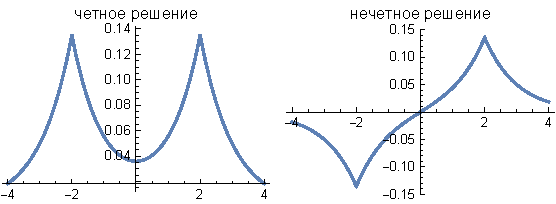
\includegraphics[width=0.5\textwidth]{figures/T5.pdf}
    \caption{Четное и нечётное решение к Т5}
\end{figure}
\textbf{Нормировка}. Для нахождения волновой функции, найдём коэффициент $A$ из нормируемости на 1:
\begin{align*}
    \int_{-\infty}^{+\infty} |\psi_+(x)|^2 \d x &= 1,
    \hspace{0.5cm} \Rightarrow \hspace{0.5cm}
    A_+^2 = \frac{\kappa}{2} \frac{(1 + e^{2 a \kappa})^2}{1 + e^{2 a \kappa} + 2 a \kappa} \\
    \int_{-\infty}^{+\infty} |\psi_-(x)|^2 \d x &= 1,
    \hspace{0.5cm} \Rightarrow \hspace{0.5cm}
    A_-^2 = \frac{\kappa}{2} \frac{(-1 + e^{2 a \kappa})^2}{-1 + e^{2 a \kappa} - 2 a \kappa} 
\end{align*}
Таким образом нашли собственные функции к этой задаче. 


Стоит вспомнить, что уравнение \eqref{T5} -- трансцендентное уравнение, где $\kappa = \kappa(E)$, то есть уравнение на уровни энергии. Как мы показали, $\kappa_+$ соответствует четному решению и $\kappa_-$ нечётному, из достаточно убедительного рисунка\footnote{
    Где по Ox отложена $\kappa \sim \sqrt{E}$, оси действительно полезно подписывать.
}  №\ref{fig:T52} видно, что $E^+ > E^-$. 


\begin{figure}[ht]
    \centering
    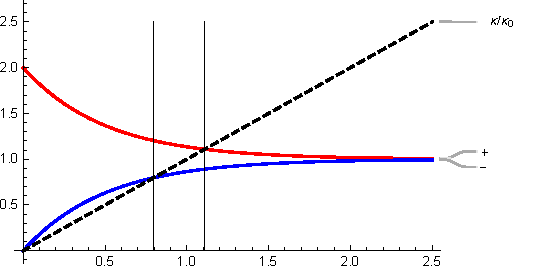
\includegraphics[width=0.5\textwidth]{figuresT5_fig2.pdf}
    \caption{Решение трансцендентного уравнения к Т5}
    \label{fig:T52}
\end{figure}


\textbf{Далекие ямы}. Рассмотрим предельный случай $\kappa_0 a \gg 1$, соответствующий достаточно далёким ямам, тогда $\kappa_+ \approx \kappa_- \approx \kappa_0$, то есть система вырождается по энергии. 


\textbf{Вероятность перехода}. В силу существования чётного и нечётного решения, можем построить состояния, соответствующие нахождению в правой ($\psi_a$) и левой ($\psi_{-a}$) ямах:
\begin{equation*}
    \left\{\begin{aligned}
        \psi_a &= \tfrac{1}{\sqrt{2}} \big( \psi_+ + \psi_- \big); \\
        \psi_a &= \tfrac{1}{\sqrt{2}} \big( \psi_+ - \psi_- \big);
    \end{aligned}\right.
    \hspace{0.5cm} \Rightarrow \hspace{0.5cm}
    \left\{\begin{aligned}
        \psi_+ &= \tfrac{1}{\sqrt{2}} \big( \psi_a + \psi_{-a} \big);\\
        \psi_- &= \tfrac{1}{\sqrt{2}} \big( \psi_a - \psi_{-a} \big).\\
    \end{aligned}\right.
\end{equation*}
Теперь, из уравнения Шрёдингера, найдём эволюцию во времени для собственных состояний:
\begin{equation*}
    i \hbar \partial_t \psi = \hat{H} \psi = - E \psi,
    \hspace{0.5cm} \Rightarrow \hspace{0.5cm}
    \psi_+ (x, t) = e^{- \frac{i}{\hbar} E_+ t} \psi_+(x),
    \hspace{5 mm} 
    \psi_- (x, t) = e^{- \frac{i}{\hbar} E_- t} \psi_-(x).
\end{equation*}
Для состояния $\psi_a$ найдём зависимость от времени в базисе $\psi_a,\, \psi_{-a}$:
\begin{equation*}
    \psi_a (x, t) = 
    \frac{1}{\sqrt{2}} (\psi_+(x, t) + \psi_- (x, t)) = 
    \frac{1}{2} \left(
        \psi_a(x) \left(
            e^{-i E^+ t / \hbar} + e^{- i E^- t / \hbar}
        \right) + \psi_{-a}(x) \left(
            e^{-i E^+ t / \hbar} - e^{-i E^- t / \hbar}
        \right)
    \right).
\end{equation*}
Вероятность перехода можем найти, как
\begin{equation*}   
    P = | \bk{\psi_{a}(x, t)}{\psi_{-a}(x)}|^2 = \bigg|
        \frac{1}{2} \underbrace{\left(
            \int |\psi_{-a}|^2 \d x
        \right)}_{\equiv 1} \left(
            e^{- i E^+ t / \hbar} - e^{-i E^- t / \hbar}
        \right)
    \bigg|^2 = \sin^2 \left(
        \frac{E^+ - E^-}{2 \hbar} t
    \right).
\end{equation*}
Можем чуть более явно найти вероятность, считая $\kappa_0 a \gg 1$, тогда
\begin{equation*}
    \kappa_+^2 \approx \kappa_0^2 + \frac{2 \kappa_0^2}{e^{2 \kappa_0 a}}, 
    \hspace{5 mm} 
    \kappa_-^2 \approx \kappa_0^2 - \frac{2 \kappa_0^2}{e^{2 \kappa_0 a}}, 
    \hspace{0.5cm} \Rightarrow \hspace{0.5cm}
    P = \sin^2 \left(
        \frac{\kappa_0^2 \hbar}{m} e^{- 2 \kappa_0 a} t
    \right).
\end{equation*}
